\chapter{Infrastructure}\label{chap:infrastructure}

% WHAT is infrastructure

% WHY is infrastructure (the purpose of it)
%    Importance of automation: builds, testing, deployment
%    Requirements: WHY we spent time doing this

% HOW is infrastructure
%    Tooling!

Broadly, infrastructure tools fit into one or more of four categories:
building, testing, deployment, and task automation.


\section{Building}

% TODO: Pre-processing and cache busting

% Content hashing case study with autotools
\cite{kelly2002optimization}


\subsection{Autotools}

% TODO: Novel application of autotols for websites

% Literate configure.ac

%%%%%%%%%%%%%%%%%%%%%%%%%%%%%%%%%%%%
%% Figure: build-system-flowchart %%
%%%%%%%%%%%%%%%%%%%%%%%%%%%%%%%%%%%%
\begin{figure}[H]
\centering
\begin{tikzpicture}[auto, thick,
                    scale=0.65, every node/.style={scale=0.65},
                    node distance = 2cm]

  % HTML NODES:
  \node (start) [block] {\textbf{START}};
  \node (more-html) [decision, below of=start] {More HTML targets?};
  \node (html-next) [block, below of=more-html] {Get next HTML target};
  \node (html-modified) [decision, below of=html-next] {Source modified?};
  \node (html-compile) [block, below of=html-modified] {Compile HTML};
  \node (html-update) [block, left of=html-compile] {Update timestamp};

  % HTML EDGES:
  \draw[->] (start) -- (more-html);
  \draw[->] (more-html) -- node {YES} (html-next);
  \draw[->] (html-next) -- (html-modified);
  \draw[->] (html-modified) -- node {YES} (html-compile);
  \draw[->] (html-compile) -- (html-update);
  \draw[->] (html-modified.180) -- node {NO} ++ (-1.65,0);
  \draw[->] (html-update) |- (more-html.180);

  % CSS NODES:
  \node (more-css) [decision, right of=more-html,
                    xshift=6cm] {More CSS targets?};
  \node (css-next) [block, below of=more-css] {Get next CSS target};
  \node (css-modified) [decision, below of=css-next] {Source modified?};
  \node (css-html) [decision, left of=css-modified,
                    xshift=-0.2cm] {HTML modified?};
  \node (css-compile) [block, below of=css-modified] {Compile CSS};
  \node (css-update) [block, left of=css-compile,
                      xshift=-2.4cm] {Update timestamp};
  \node (css-ref) [block, above of=css-update,
                   yshift=3cm] {Update HTML references};

  % CSS EDGES:
  \draw[->] (more-html.0) -- node {NO} ++ (1, 0) -- (more-css);
  \draw[->] (more-css) -- node {YES} (css-next);
  \draw[->] (css-next) -- (css-modified);
  \draw[->] (css-modified) -- node {YES} (css-compile);
  \draw[->] (css-modified) -- node {NO} (css-html);
  \draw[->] (css-compile) -- (css-update);
  \draw[->] (css-update) -- (css-ref);
  \draw[->] (css-ref) |- (more-css);
  \draw[->] (css-html) -- node {NO} ++ (0, 2) |- (more-css);
  \draw[->] (css-html.180) -- node {YES} ++ (-.85cm, 0);

  % JS NODES:
  \node (more-js) [decision, right of=more-css,
                    xshift=6cm] {More JS targets?};
  \node (js-next) [block, below of=more-js] {Get next JS target};
  \node (js-modified) [decision, below of=js-next] {Source modified?};
  \node (js-html) [decision, left of=js-modified,
                    xshift=-0.2cm] {HTML modified?};
  \node (js-compile) [block, below of=js-modified] {Compile JS};
  \node (js-update) [block, left of=js-compile,
                      xshift=-2.4cm] {Update timestamp};
  \node (js-ref) [block, above of=js-update,
                   yshift=3cm] {Update HTML references};
  \node (finish) [block, above of=more-js] {\textbf{FINISH}};

  % JS EDGES:
  \draw[->] (more-css.0) -- node {NO} ++ (1, 0) -- (more-js);
  \draw[->] (more-js) -- (finish);
  \draw[->] (more-js) -- node {YES} (js-next);
  \draw[->] (js-next) -- (js-modified);
  \draw[->] (js-modified) -- node {YES} (js-compile);
  \draw[->] (js-modified) -- node {NO} (js-html);
  \draw[->] (js-compile) -- (js-update);
  \draw[->] (js-update) -- (js-ref);
  \draw[->] (js-ref) |- (more-js);
  \draw[->] (js-html) -- node {NO} ++ (0, 2) |- (more-js);
  \draw[->] (js-html.180) -- node {YES} ++ (-.85cm, 0);
\end{tikzpicture}
\caption[Build system flowchart]{Build system flowchart.}
\label{fig:build-system-flowchart}
\end{figure}

\newpage

%%%%%%%%%%%%%%%%%%%%%%%%%%%%%%%
%% Listing: build-javascript %%
%%%%%%%%%%%%%%%%%%%%%%%%%%%%%%%
\lstset{language=make}
\begin{lstlisting}[label=lst:build-javascript,caption={
      [Autotools Makefile pattern for JavaScript compilation]
      Autotools Makefile pattern for JavaScript compilation, taken
      from \texttt{www/js/Makefile.am}. The conditional variables
      \texttt{ENABLE\_MINI\_JS} and
      \texttt{ENABLE\_CONTENT\_HASHING} are used to control the
      behaviour of the compilation, and are set by passing argument
      flags to the configuration script.}]
# Compilation command
if ENABLE_MINIFY_JS
define compile
  $(JAVA) -jar $(JS_JAR) --js=$1 --js_output_file=$2
endef
else # Disabled minification
define compile
  cat $1 > $2
endef
endif

# JavaScript compilation
$(DEST)/%.js: %.js
  @test -d $(DEST) || { \
    $(MKDIR_P) $(DEST); \
  }
if ENABLE_CONTENT_HASHING
  $(eval CHASH := $(shell $(HASH_BIN) $< | cut -c1-$(HASH_LENGTH)))
  $(eval NAME := $(addsuffix -$(CHASH).js,$(patsubst %.js,%,$@)))
else
  $(eval NAME := $@)
endif
  @test -f $(NAME) || { \
    echo '  JS     $(notdir $(NAME))'; \
    $(call compile,$<,$(NAME)); \
  }
if ENABLE_CONTENT_HASHING
  $(eval TARGET := js\/$(patsubst %.js,%,$<))
  @for h in $(HTML); do \
    sed -ri 's/(<script src=\"(\{\{ *(\w|[_.])+ *\}\})*\/?)$(TARGET)(-[0-9a-f]{$(HASH_LENGTH)})?(\.js\")/\1$(TARGET)-$(CHASH)\5/' $$h; \
  done
endif
\end{lstlisting}

\subsubsection*{Build system parallelisation}


%%%%%%%%%%%%%%%%%%%%%%%%%
%% Figure: build-times %%
%%%%%%%%%%%%%%%%%%%%%%%%%
\begin{figure}[H]
\centering
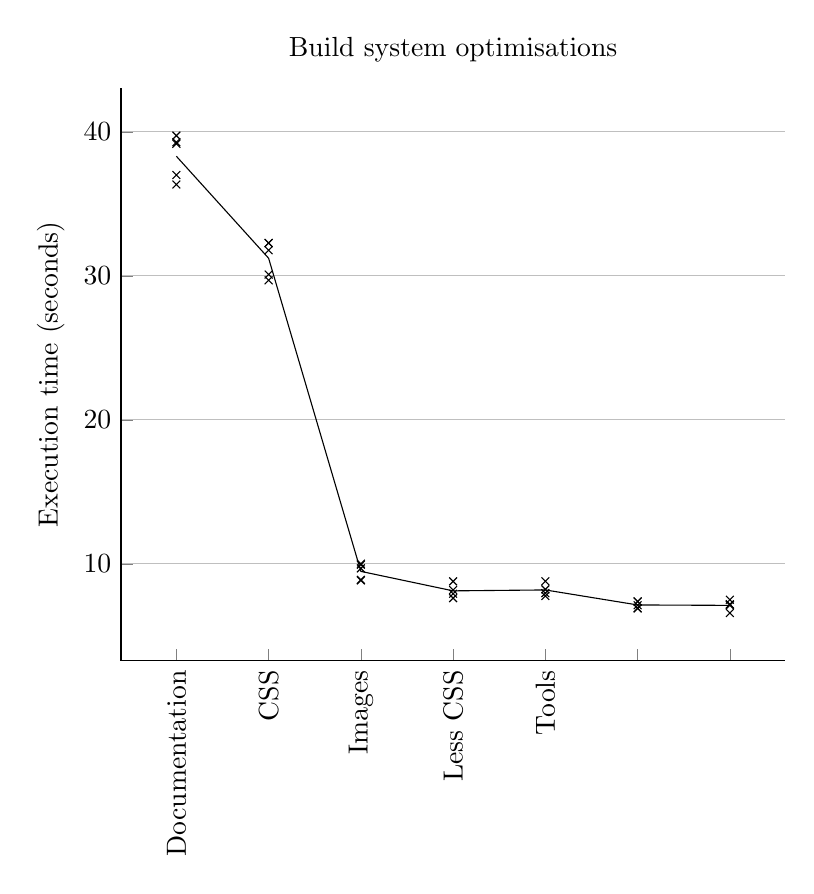
\begin{tikzpicture}
\begin{axis}[
    title={Build system optimisations},
    axis y line*=left,
    axis x line*=bottom,
    scale only axis,
    ymajorgrids,
    xticklabels={Control,
                 JavaScript,
                 Documentation,
                 CSS,
                 Images,
                 Less CSS,
                 Tools},
    x tick label style={rotate=90,anchor=east},
    ylabel={Execution time (seconds)}
  ]
% PLOT: Results
\addplot+[only marks,
          mark options={color=black},
          mark=x
]
coordinates{
  (1,39.169)
  (1,37.001)
  (1,36.344)
  (1,39.74)
  (1,39.276)
  (2,32.287)
  (2,29.689)
  (2,30.088)
  (2,31.775)
  (2,32.275)
  (3,8.887)
  (3,8.849)
  (3,9.68)
  (3,9.937)
  (3,10.007)
  (4,8.176)
  (4,8.777)
  (4,7.918)
  (4,7.614)
  (5,7.761)
  (5,8.788)
  (5,8.222)
  (5,7.96)
  (6,6.915)
  (6,6.9)
  (6,7.121)
  (6,7.38)
  (6,7.385)
  (7,6.582)
  (7,7.128)
  (7,7.192)
  (7,7.159)
  (7,7.498)
};
% PLOT: Best fit line
\addplot+[mark=none,
          color=black
]
coordinates {
  (1,38.306)
  (2,31.2228)
  (3,9.472)
  (4,8.1195)
  (5,8.18275)
  (6,7.1402)
  (7,7.1114)
};
\end{axis}
\end{tikzpicture}
\caption[Graph of build system execution times with optimisations]
        {Graph of build system execution times after each optimisation
          iteration. Each value is sequential, with the leftmost
          control value being the execution time of the unmodified
          serial build system. The tests were invoked with the command
          \texttt{time (./autogen.sh \&\& ./configure \&\& make)}.}
\label{fig:build-times}
\end{figure}


\subsection{On-demand compilation using inotify subsystem}

\cite{love2005kernel, shields2010inotify}


\section{Testing}

% AUTOMATED TEST COVERAGE
\cite{zhu1997software}

% TEST COVERAGE
\cite{woodward1980experience, gupta2000generating}

\subsection{Branch analysis for test coverage}


% Cloverage

\subsection{Continuous integration}


% Travis CI

\section{Deployment}

% Continuous integration:

\cite{fowler2006continuous, duvall2007continuous}

% Heroku


\section{Task automation}\label{sec:task-automation}

% TODO: brief explanation of each script in scripts/


\subsection{dsa: Dataset analysis}

% TODO: dsa


%%%%%%%%%%%%%%%%%%%%%%%%%%%
%% Figure: dsa-populated %%
%%%%%%%%%%%%%%%%%%%%%%%%%%%
\begin{figure}[H]
\centering
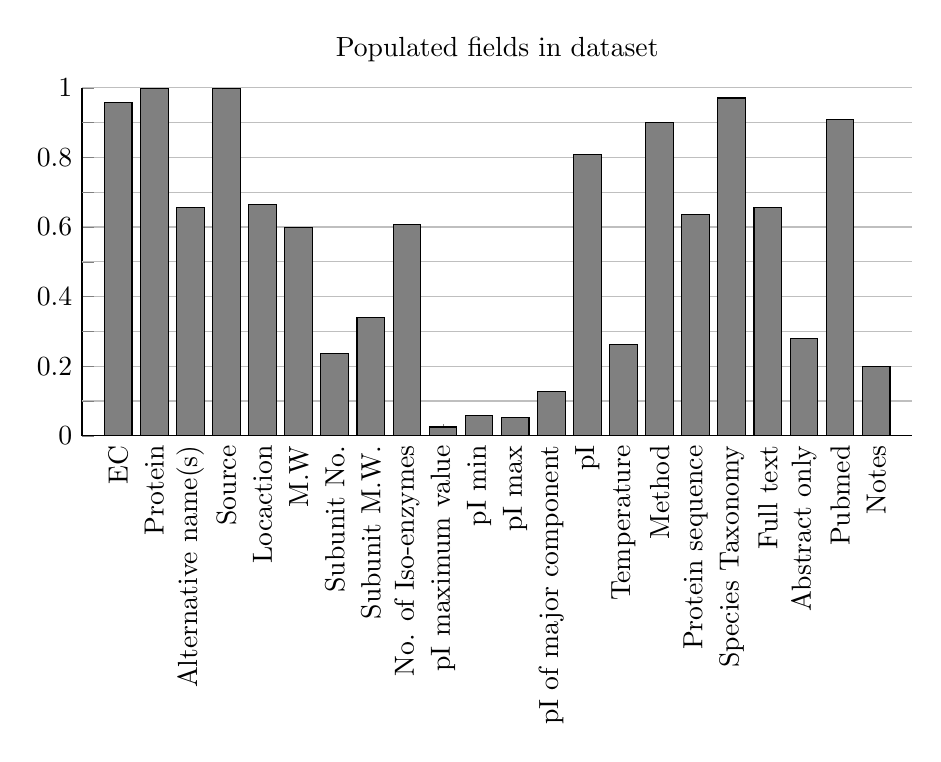
\begin{tikzpicture}
\begin{axis}[%
    title={Populated fields in dataset},
    width=\textwidth, height=6cm,
    axis y line*=left,
    axis x line*=bottom,
    ymin=0, ymax=1,
    xmin=0, xmax=23,
    extra y tick style={yticklabels={}},
    extra y ticks={0.1,0.3,0.5,0.7,0.9},
    ymajorgrids,
    x tick label style={rotate=90,anchor=east},
    xtick=data,
    xticklabels={%
      EC,
      Protein,
      Alternative name(s),
      Source,
      Locaction,
      M.W,
      Subunit No.,
      Subunit M.W.,
      No. of Iso-enzymes,
      pI maximum value,
      pI min,
      pI max,
      pI of major component,
      pI,
      Temperature,
      Method,
      Protein sequence,
      Species Taxonomy,
      Full text,
      Abstract only,
      Pubmed,
      Notes
    }
  ]
% PLOT: Results
\addplot+[%
  ybar,
  no marks,
  fill=gray,
  draw=black
]
plot coordinates{
  (1,0.957402597)
  (2,0.999134199)
  (3,0.656277056)
  (4,0.999307359)
  (5,0.665108225)
  (6,0.598961039)
  (7,0.237056277)
  (8,0.340952381)
  (9,0.606060606)
  (10,0.025281385)
  (11,0.057142857)
  (12,0.053333333)
  (13,0.127965368)
  (14,0.807965368)
  (15,0.262683983)
  (16,0.90025974)
  (17,0.635844156)
  (18,0.970909091)
  (19,0.656796537)
  (20,0.280692641)
  (21,0.909437229)
  (22,0.198614719)
};
\end{axis}
\end{tikzpicture}
\caption[Populated fields in dataset]
        {The proportion of populated keys for each field in the dataset.}
\label{fig:dsa-populated}
\end{figure}


\newpage
\subsection{png: Generation of test data}

% TODO: novel application of Markov text generators for creating
% plausible scientific data for testing purposes.

\cite{atwood2008markov, page1999pagerank}

% TODO: png


%%%%%%%%%%%%%%%%%%%%%%%%%%%
%% Listing: markov-chain %%
%%%%%%%%%%%%%%%%%%%%%%%%%%%
\lstset{language=JavaScript}
\begin{lstlisting}[label=lst:markov-chain,caption={%
      [Markov chain implementation]
      Markov chain implementation in JavaScript.}]
for (var i = 0; i < list.length; i++) {
  var sentence = list[i].split(' ');

  terminals.push(sentence[sentence.length - 1]);
  startwords.push(sentence[0]);

  for (var j = 0; j < sentence.length - 1; j++) {
    var nextWord = sentence[j + 1];

    if (wordTrees[sentence[j]] !== undefined)
      wordTrees[sentence[j]].push(nextWord);
    else
      wordTrees[sentence[j]] = [nextWord];
  }
}
\end{lstlisting}


%%%%%%%%%%%%%%%%%%%%%%%%%%%%%%%%%%%%
%% Listing: markov-text-generator %%
%%%%%%%%%%%%%%%%%%%%%%%%%%%%%%%%%%%%
\lstset{language=JavaScript}
\begin{lstlisting}[label=lst:markov-text-generator,caption={%
      [Markov text generator]
      Markov text generator implementation.}]
var next = function() {
  var word = rand(startwords);
  var sentence = [word];

  while (wordTrees[word] !== undefined) {
    var nextWords = wordTrees[word];

    word = rand(nextWords);
    sentence.push(word);

    if (terminals[word] !== undefined)
      break;
  }

  return sentence.join(' ');
};
\end{lstlisting}


\newpage
\subsection{pipbot: Task automation}\label{sec:pipbot}


%%%%%%%%%%%%%%%%%%%%%%%%%
%% Figure: pipbot-logo %%
%%%%%%%%%%%%%%%%%%%%%%%%%
\begin{figure}[H]
\begin{verbatim}
                              ,--.    ,--.
                             ((O ))--((O ))
                           ,'_`--'____`--'_`.
                          _:  ____________  :_
                         | | ||::::::::::|| | |
                         | | ||::::::::::|| | |
                         | | ||::::::::::|| | |
                         |_| |/__________\| |_|
                           |________________|
                        __..-'            `-..__
                     .-| : .----------------. : |-.
                   ,\ || | |\______________/| | || /.
                  /`.\:| | ||  __  __  __  || | |;/,'\
                 :`-._\;.| || '--''--''--' || |,:/_.-':
                 |    :  | || .----------. || |  :    |
                 |    |  | || '--pipbot--' || |  |    |
                 |    |  | ||   _   _   _  || |  |    |
                 :,--.;  | ||  (_) (_) (_) || |  :,--.;
                 (`-'|)  | ||______________|| |  (|`-')
                  `--'   | |/______________\| |   `--'
                         |____________________|
                          `.________________,'
                           (_______)(_______)
                           (_______)(_______)
                           (_______)(_______)
                           (_______)(_______)
                          |        ||        |
                          '--------''--------'
                     Hello there. My name is pipbot.
\end{verbatim}
\caption[The pipbot welcome message]
  {The pipbot welcome message, displayed at the start of interactive sessions.}
\label{fig:pipbot-logo}
\end{figure}


%%%%%%%%%%%%%%%%%%%%%%%%%%%%
%% Figure: pipbot-session %%
%%%%%%%%%%%%%%%%%%%%%%%%%%%%
\begin{figure}[H]
\begin{verbatim}
$ pipbot
Hello there. My name is pipbot.
-> burndown 7 days
Comparing `master' against `master'...

  There are 56 new commits on master
  The last commit on master was 5 days, 2 hours ago
-> version
0.6.2
-> start 0.6.3
Summary of actions:
- A new branch release/0.6.3 was created, based on master.
- A new remote branch release/0.6.3 was created on origin.
- Branch release/0.6.3 tracks remote branch release/0.6.3 from origin.
- You are now on branch release/0.6.3.
- The version  number has been bumped to 0.6.3 and committed

Now, start performing release fixes. When done, use:

     pipbot finish 0.6.3

-> exit
Goodbye!
\end{verbatim}
\caption[Example pipbot session]
  {An example pipbot interactive session, in which the user begins a
   new release. User issued commands begin with the prefix
   ``\texttt{-> }''. First, the user requests a burndown of the
   repository activity over the past week; then they request the
   current version, and begin a new release with the version number
   \texttt{0.6.3}.}
\label{fig:pipbot-session}
\end{figure}
